\documentclass[conference]{IEEEtran}
\IEEEoverridecommandlockouts
% The preceding line is only needed to identify funding in the first footnote. If that is unneeded, please comment it out.
\usepackage{cite}

\usepackage{amsmath,amssymb,amsfonts}
\usepackage{algorithmic}
\usepackage{graphicx}
\usepackage{textcomp}
\usepackage{xcolor}

\DeclareGraphicsExtensions{.pdf,.jpeg,.png,.eps}
\graphicspath{{./figures/}}

\usepackage{multirow}

\usepackage{colortbl}


    
\begin{document}

\title{IEEE 802.15.4 Historical Evolution and Trends}
\author{\IEEEauthorblockN{1\textsuperscript{st} Alberto Gallegos Ramonet}
\IEEEauthorblockA{\textit{College of Information Science and Engineering} \\
\textit{Ritsumeikan University}\\
Shiga, Japan }
\and
\IEEEauthorblockN{2\textsuperscript{nd} Taku Noguchi}
\IEEEauthorblockA{\textit{College of Information Science and Engineering} \\
\textit{Ritsumeikan University}\\
Shiga, Japan}
}

\maketitle

\begin{abstract}
For several years the IEEE 802.15.4 standard has been the backbone in applications with low latency and small energy consumption requirements. Its popularity is such that this standard has become de facto standard for this type of network communications and will keep playing an important role in the Internet of Things (IoT) revolution. The standard is 15 years old and both, its reach and purpose have changed over the years. In this paper, we present a concise and chronological description of the standard highlighting each one of the introduced features over the years. A compendium like this one, is valuable for researchers working on implementations and improvements as well as users looking for a general reference. This is relevant now more than ever because the standard must coexist with hundreds of other standards which are also in constant evolution. As shown in this document and despite its popularity and importance, the number of available IEEE 802.15.4 capable simulators are very reduced and often, outdated and incomplete. Our goal with this paper is to provide a quick reference but also show the standard evolution and future direction. At the same time, we hope this work foster the creation of new implementations, particularly new simulations modules.
 
\end{abstract}

\begin{IEEEkeywords}
LR-WPAN, protocols, survey, WSN, simulations, Zigbee, IEEE 802.15.4
\end{IEEEkeywords}

\section{Introduction}
From the networks in our homes and offices, to the networks of our mobile devices, networks are always in constant evolution. Not all network enabled devices are connected to the Internet nor they need to be. For example, devices found in our homes such as electric doors, televisions and air conditioning systems, may benefit from sharing information between each other, but in most of the cases using internet to connect these appliances may not be a cost effective solution because of the unnecessary added complexity, communication overhead and unwanted privacy concerns. In these cases, internet independent networks are a good choice. For example, independent networks used in Wireless Sensor Networks (WSN). In 2003, the IEEE 802.15.4 standard was released \cite{std2003} to describe this type of networks. WSN are characterized for strict power constraints in specialized applications with low latency or prompt to disruptive connections. In this paper, we present a chronological description of the IEEE 802.15.4 standard known as Low-Rate Wireless Personal Area Networks (LR-WPAN). Furthermore, this work describe the MAC behaviors and the available options of its physical layers, as well as clarify the often overlooked formation of mesh networks and available simulations. Despite the popularity of the IEEE 802.15.4 standard, to our knowledge there are no similar compendiums summarizing a complete evolution of the standard. This document is relevant for multiple reasons. For instance, the standard include an extensive collection of physical layer options and MAC layer improvements which are not available for all the revisions. In some cases, drastic changes raise some implementations obsolete or incompatible. Moreover, official standard descriptions assume knowledge of prior revisions which makes these documents hard to navigate without having a general context of the standard such as the one presented here. As a result, new improvements and implementations are a convoluted and time consuming task. It is also worth noting that implementations and simulations of the standard are considerably behind the most recent revisions. For example, Zigbee, arguably the most popular commercial implementations of the IEEE 802.15.4 standard, only until recently (V3.0) has support for the 2011 revision of the standard \cite{nxpManual} despite the existence of amendments as late as 2018. For these reasons, we believe that users and implementers alike will find the summary presented in this document relevant. This paper is organized as follows: Section \ref{evolutionStd} describes a full evolution of the IEEE 802.15.4 standard highlighting differences between revisions. %A summary of the PHY layers conforming the standard can be located %at Table \ref{tab:phyTable} at the end of this Section. 
Section \ref{implementationStd} shows a brief description of some of most popular simulations implementations followed by our conclusions.


\section{Evolution of the IEEE 802.15.4 Std.} \label{evolutionStd}

\subsection{IEEE 802.15.4 (2003)}\label{wpan2003}

Initially released in 2003, the IEEE 802.15.4 standard \cite{std2003} defines the interconnection of LR-WPAN devices. It uses the Carrier Sense Multiple Access with a Collision Avoidance (CSMA/CA) to access the medium and support star and peer-to-peer topologies. Its architecture layout can be described in terms of blocks, based on the open systems interconnection (OSI) seven-layer model in which each block (also called layer) has an specific task and offer services to upper blocks. The PHY layer (Physical layer or layer 1) contains the radio frequency (RF) transceiver along with a low-level control mechanism. The 2003 standard defines two PHYs: a 2450 MHz direct sequence spread spectrum (DSSS) with a maximum data rate over-the-air of 250 kb/s and the less commonly used 915 Mhz and 868 Mhz bands with data rates of 40 kb/s and 20 kb/s, respectively. 
The MAC layer (Media Access Control or layer 2) provides access to the physical channel. Although the standard consists mainly of these two layers, the standard also describes an additional Logical Link Control (LLC) and a Service Specific Convergence Sublayer (SSCS) between the MAC layer and the next layer to facilitate the communication. Upper layers implementation details are beyond the scope of the standard. Transmission of data can be done with or without the help of beacon messages. In a beacon-enabled Personal Area Network (PAN), a single Full Functional Device (FFD) acts as a PAN coordinator while the rest of the devices are either FFD or Reduced Functional Devices (RFD). Different to a beacon-enabled PAN, in a non-beacon enabled PAN devices compete for the the medium at all times. 
% The popularity of the 2450MHz over the other two PHY is attributed to 3 factors: Its %higher data rate of 250 kb/s, the fact that 2450Mhz was a free spectrum  in most of the %world at the time of its release and the fact that the other two bands used a different %modulation technique which from the point of view of physical implementation presented %challenges to the sellers.
\begin{figure}[!htb]
\centering
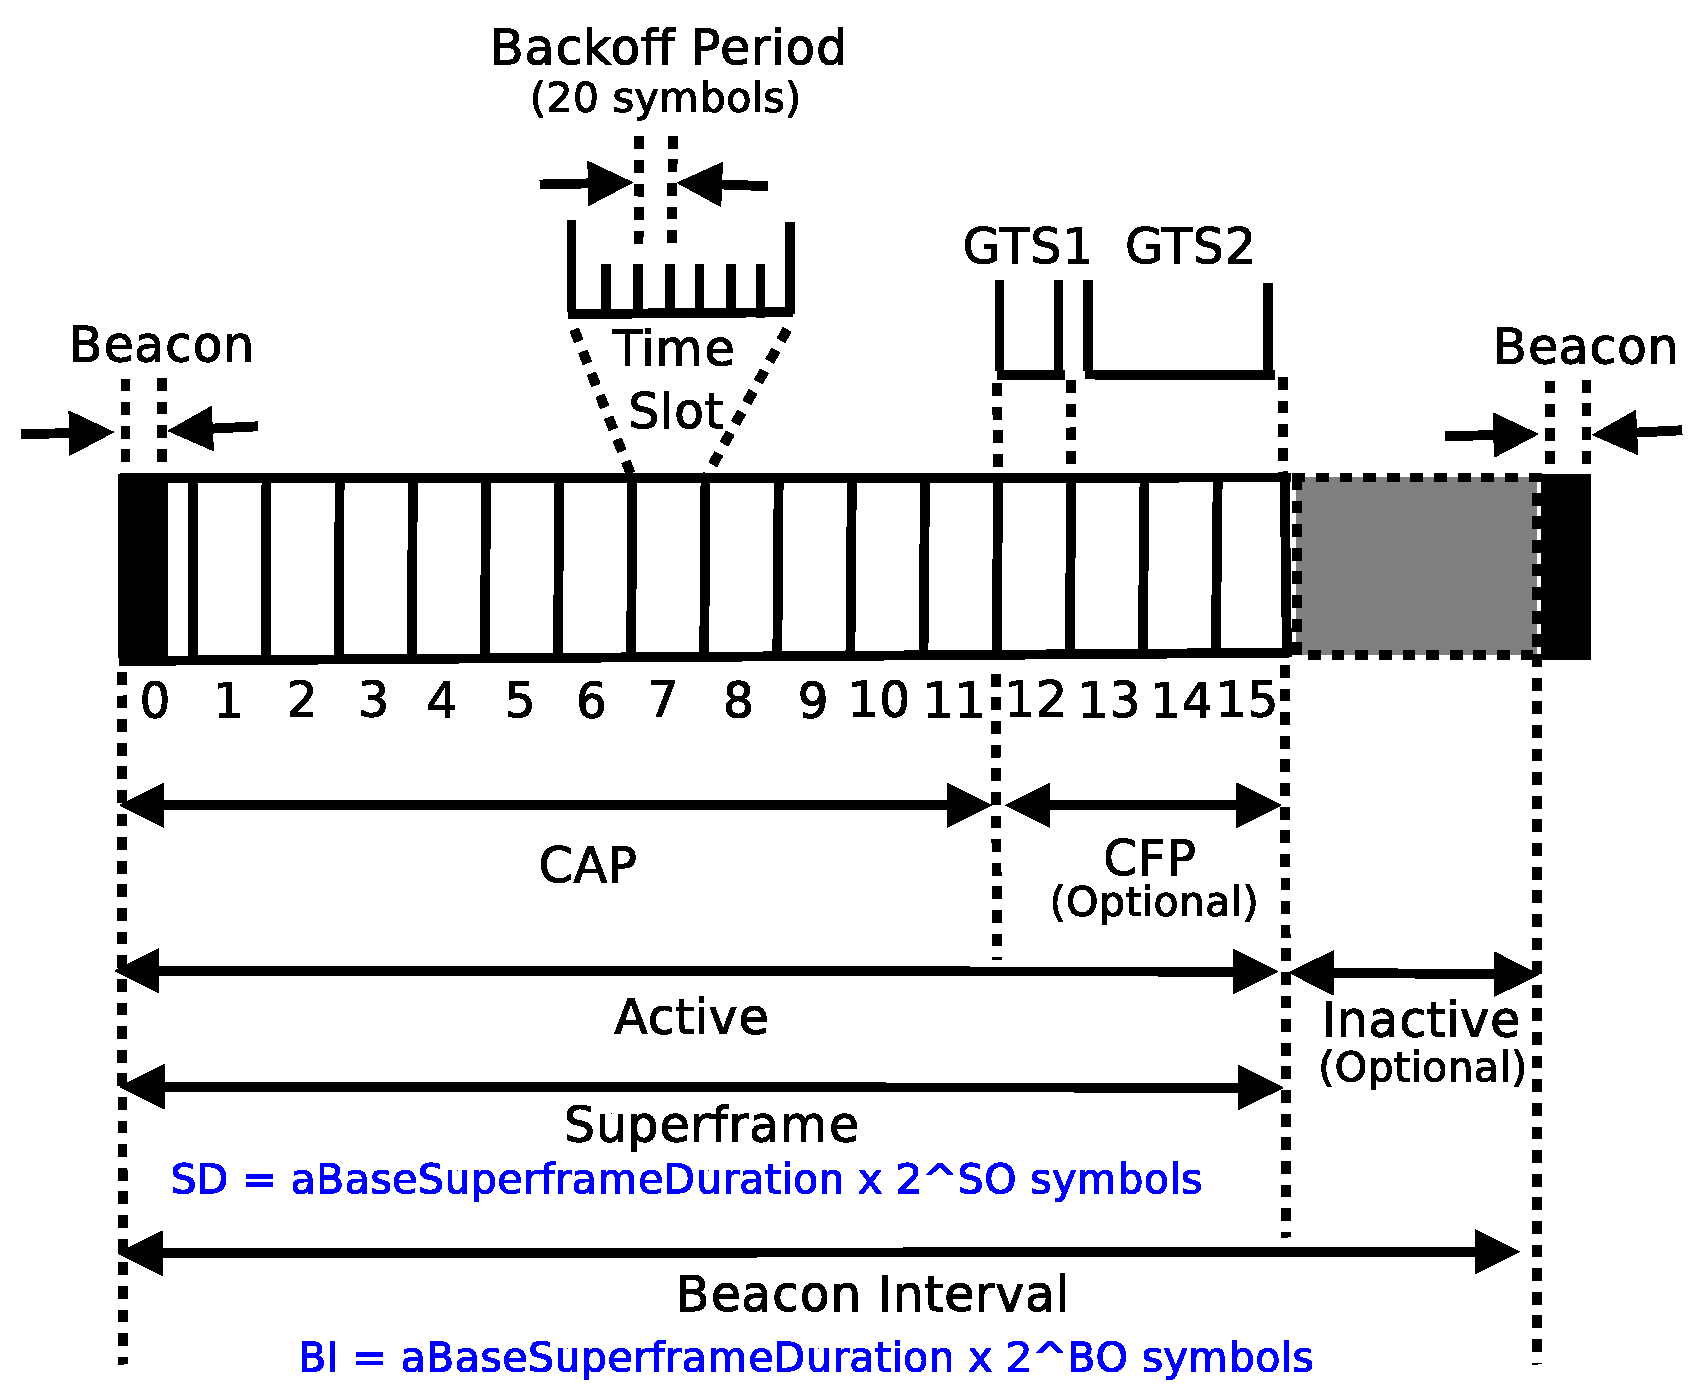
\includegraphics[scale=.28]{superframe}
\caption{Beacon-enabled mode superframe description.}
\label{fig:superframe}
\end{figure}

In a beacon-enabled PAN, the PAN coordinator transmits in intervals beacons containing a \textit{superframe} structure that defines an active period of time between beacons. The superframe is used to achieve synchronized communication between the PAN devices. Figure \ref{fig:superframe} summarizes the structure of a superframe. A superframe is formed by 16 time slots in which a beacon is always sent during the first time slot. In the same way, each of these time slots are formed by 20 \textit{symbols}. A symbol is a representation of time in bits. For example, in IEEE 802.15.4 using a O-QPSK modulation, 1 symbol is equivalent to 4 bits (0.016 ms in a 250kbps connection). A Beacon Interval (BI) is defined by  \mbox{$aBaseSuperframeDuration \times 2^{SO}$} symbols. Where Superframe Order (SO) is a user defined integer between 0 and 14 and $aBaseSuperframeDuration$ is a constant equal to 960 symbols. The BI includes both,the active and inactive periods of time. The inactive period is optional with no transmissions and where the radio transceiver can remain off to preserve energy. The active portion depends on the user defined variable Beacon Order ($BO$) and its length is described by the Superframe Duration (SD). The SD is equal to \mbox{$aBaseSuperframeDuration \times 2^{BO}$} symbols for \mbox{0 $\leq$ $SO$ $\leq$ $BO$ $\leq$ 14}. The active portion is further divided into Contention Access Period (CAP) and Contention Free Period (CFP). In the CAP, devices contend for the transmission of data using a slotted version of the CSMA/CA algorithm. Time slots are formed by multiple \textit{backoff periods} \mbox{(1 backoff period is equivalent to 20 symbols)}. Operations within the CAP always take place on the boundary of a backoff period. The CFP is an optional part of the active period but if exists, it must always be located at the end of the active period. The CFP is divided into Guaranteed Time Slots (GTS) which are assigned to specific devices to transmit without contention. A maximum of 7 GTS can be assigned. Their length depends directly on the maximum size of the CFP and the total number of GTS assigned.
\begin{figure}[!htb]
\centering
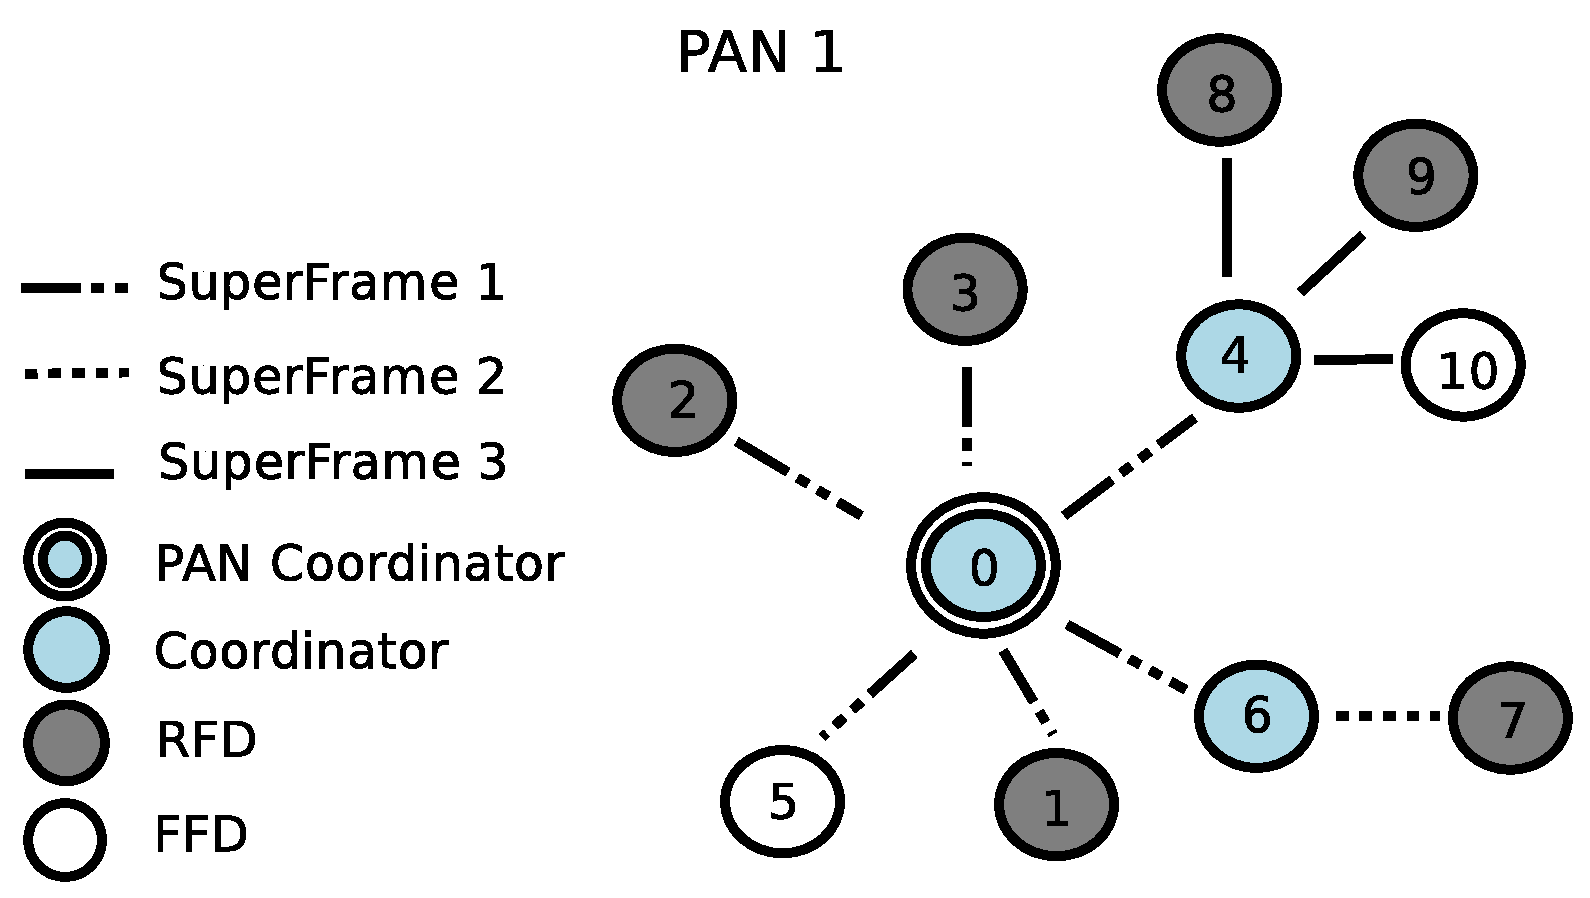
\includegraphics[scale=.28]{peerTopology}
\caption{ IEEE 802.15.4 Mesh topology in single PAN.}
\label{fig:peerTopology}
\end{figure}

\begin{figure}[!htb]
\centering
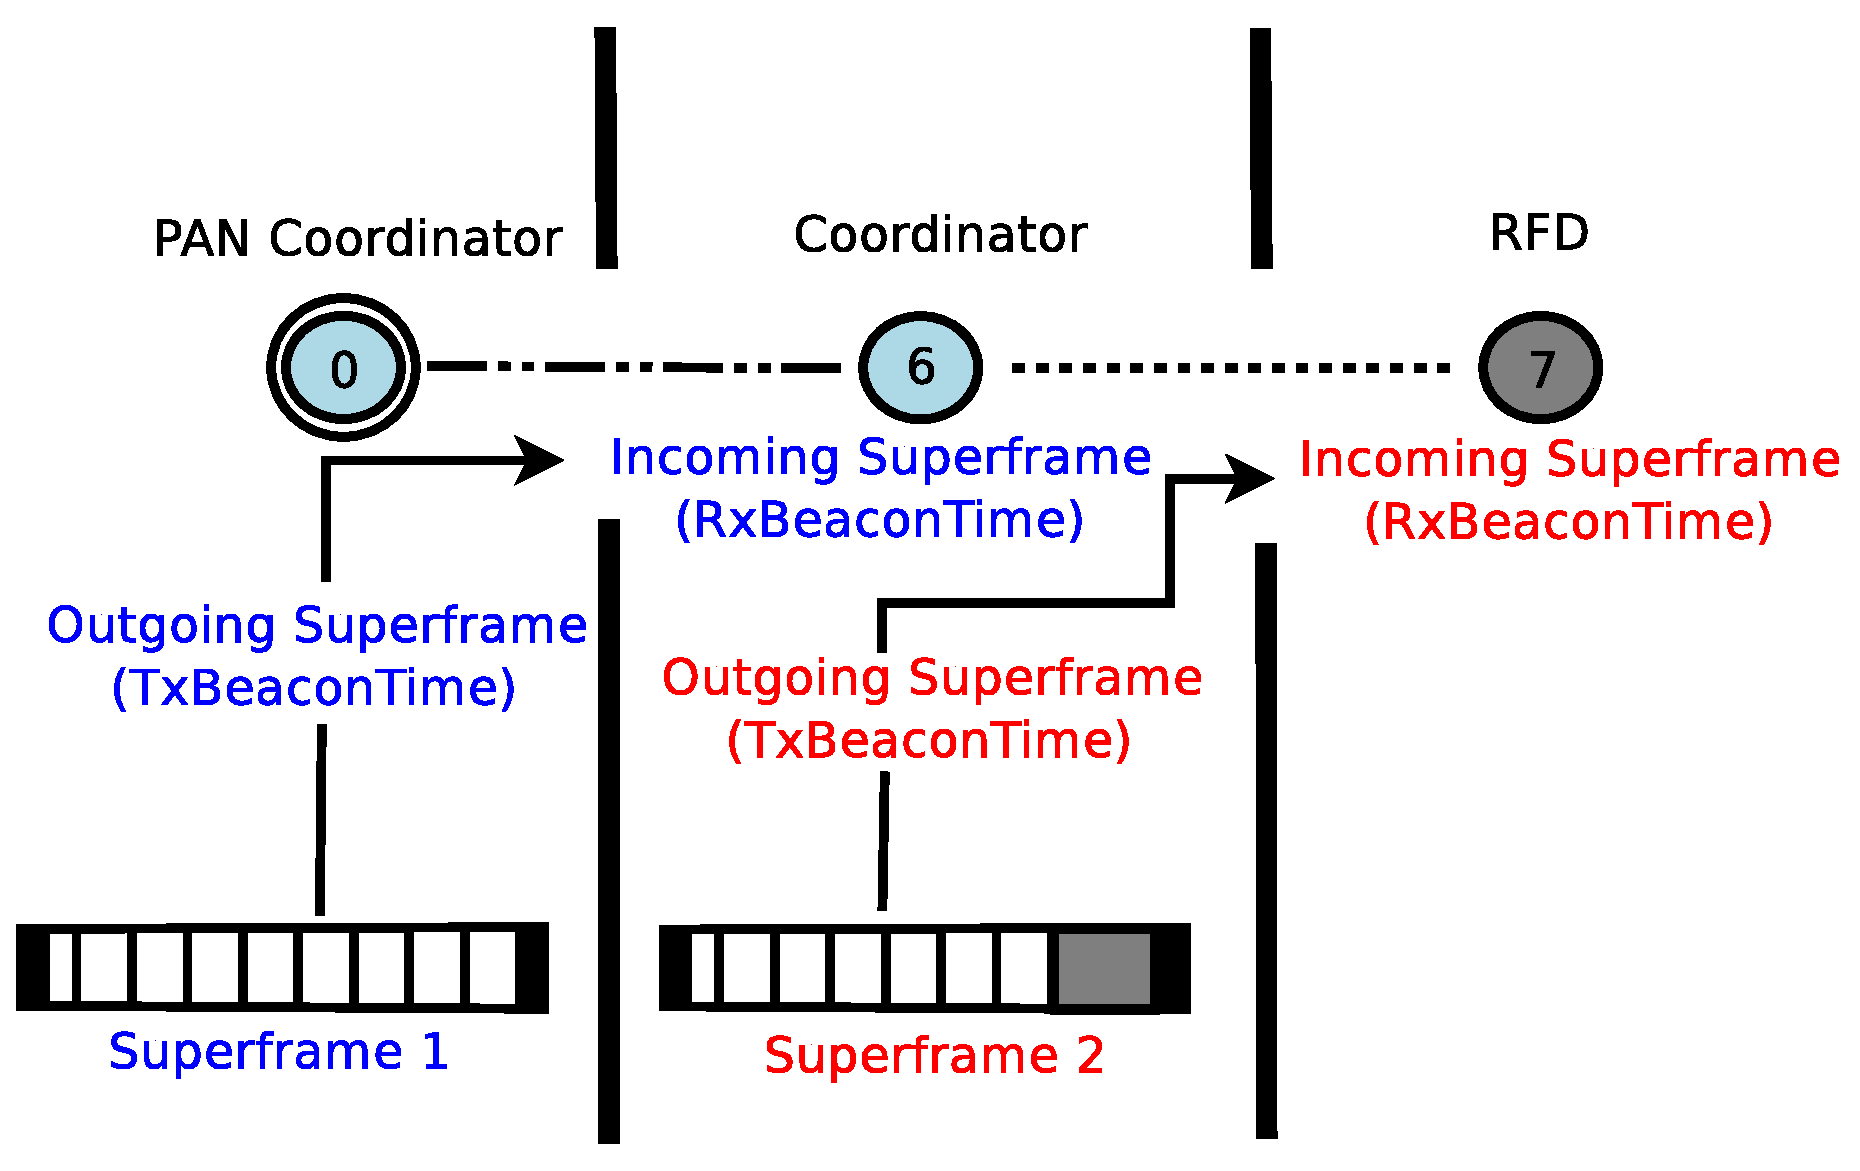
\includegraphics[scale=.28]{superframeRef}
\caption{Outgoing and Incoming superframe relationship in a Mesh Network.}
\label{fig:superframeRef}
\end{figure}

One aspect often overlooked by both, the official \mbox{IEEE 802.15.4} standard documents and researchers alike, is the beacon-enabled function in mesh topologies. While the standard states that this configuration is possible, little to no details are given on how to achieve this in its multiple revisions. Figure \ref{fig:peerTopology} shows an example on how to achieve a mesh topology. While only one PAN coordinator exists in a PAN, it is possible to have extra coordinators to create a mesh network. PAN coordinators differ from coordinators in which only PAN coordinators can initialize the network (association process) and give commands to other coordinators to administrate the network. Each coordinator transmits its own beacons containing the information of its superframe. The transmitted superframe helps to synchronize data transmissions between a coordinator and its associated devices. While in a star topology there is only one superframe at any given moment, in a mesh topology a coordinator might have to keep track of two superframes. A superframe coming from its associated PAN coordinator when it acts as a device (incoming superframe) and the superframe that it transmit to other devices when it acts as a coordinator (outgoing superframe).  In Figure \ref{fig:superframeRef}, is possible to observe this superframe relationship for one segment of the mesh network previously showed in Figure \ref{fig:peerTopology}. When the \mbox{coordinator 6} wishes to transmit data to its PAN coordinator 0, it uses the incoming superframe information \mbox{(superframe 1)}. In the same way, if \mbox{coordinator 6} wishes to transmit data to its associated device \mbox{node 7}, It will use the outgoing superframe reference that originated from itself \mbox{(superframe 2)}. An incoming superframe uses the beacon reception time from its coordinator (RxBeaconTime) as a reference for the beginning of the superframe. An outgoing superframe uses its beacon transmission time (TxBeaconTime) as a reference for the beginning of the superframe.

\subsection{IEEE 802.15.4 (2006)}\label{wpan2006}
The 2006 revision \cite{std2006} is the first revision after the standard introduction in 2003. In this revision, a field in the Frame Control Field (FCF) of the MAC Header was added to easily check the version in use. The biggest changes in this revision are in the physical layer. The 2003 original 868/915 MHz bands employed a Binary Phase-Shift Keying (BPSK) modulation. Optionally, in this revision is now possible to use an Amplitude Shift Keying (ASK) modulation on the 868/915 MHz bands. This modulation effectively increases the offered data rate to 250 kb/s for both bands. The same data rate was only previously reachable on the 2450 MHz band in the 2003 revision. Besides the 868/915 MHz bands BPSK and ASK modulations, the Optional Offset Quadrature Phase-Shift Keying (O-QPSK) modulation was added. This modulation offers an increased data rate of 100 kb/s and 250 kb/s respectively when compared to the original BPSK modulation. O-QPSK modulation was only possible with the 2450 MHz band in the 2003 revision. As for MAC layer enhancements, the 2006 revision allows the specification beacons start times via a parameter in the MAC layer primitives. Pre-establishing the start time helps to reduce the beacon collisions among PAN coordinators.

\subsection{IEEE 802.15.4a (2007) - Amendment 1}\label{wpan2007}
IEEE 802.15.4a \cite{std2007} is the first amendment to the 2006 revision. It introduces two new PHYs: the Ultra-wide Band (UWB) and the Chirp Spread Spectrum (CSS). UWB operates at frequencies 3 GHz, 5 GHz, 6 GHz to 10 GHz and less than 1 GHz (16 channels). UWB has a maximum over-the-air data rate of 851 kb/s with optional data rates of 110 kb/s, 6.81 Mb/s and 27.24 Mb/s using a combined modulation of Burst Position Modulation (BPM) and BPSK. On the other hand, CSS operates in the PHY 2450 MHz with supports for data rates of 1000 kb/s or 250 kb/s. The UWB allows the use of precision ranging (calculation of  the distance between two devices) using the Two-Way Ranging (TWR) protocol which allows the ranging calculation without the need for a common time reference.

\subsection{IEEE 802.15.4c (2009) - Amendment 2}\label{wpan2009c}
The second amendment\cite{std2009c} to the 2006 revision adds two extensions to the physical layer: One 780 MHz PHY with the O-QPSK modulation and another 780MHz PHY with the new modulation M-ary Phase Shift Keying (MPSK). Both of these additions are meant to be used in China and have a maximum data rate of 250 kb/s regardless the modulation used. 

\subsection{IEEE 802.15.4d (2009) - Amendment 3}\label{wpan2009d}
Similar to 2nd, the 3rd amendment to the 2006 revision \cite{std2009d} adds extensions to the physical layer but now exclusively for Japan. Two more PHY were added, a PHY in the 950 MHz band with a Gaussian Frequency-Shift Keying (GFSK) modulation with maximum data rate of 100 kb/s and a PHY in the 950 MHz band using the BPSK modulation with a data rate of 20 kb/s.
\subsection{IEEE 802.15.4 (2011)}\label{wpan2011}
The 2011 revision \cite{std2011} put together into a single document all changes done in the last 3 amendments after the 2006 revision. In this revision, the standard dropped the concept of Service Specific Convergence Sublayer (SSCS) focusing instead on PHY and MAC layer topics exclusively. Due to the lack of a flexible MAC layer,  the 2011 revision gave birth to numerous alternative MAC layers proposal that could fulfill the requirements of different type of applications. In time, the standard addressed these concerns and officially introduce variants to the MAC layers in the form of \textit{MAC behaviors} in subsequent amendments.

\subsection{IEEE 802.15.4e (2012) - Amendment 1}\label{wpan2012e}
While most the amendments prior this one focus on PHY layer additions, IEEE 802.15.4e\cite{std2012e} proposed significant changes to the MAC layer. These changes impacted the standard in 2 ways: First, it relegated the previous MAC layer to a all purpose legacy status. Second, it reworked the MAC layer to a modular and specialized design in the form of \textit{MAC behaviors}. These MAC behaviors bring a level of flexibility never present in the previous versions and ,therefore, represent a point of interest often surveyed and evaluated by researchers \cite{nutshell}. IEEE 802.15.4e describe 5 MAC behaviors: 
%Radio Frequency Identification (RFID) BLINK, Asynchronous Multichannel Adaptation (AMCA), %Deterministic Synchronous Multichannel Extension (DSME), Low Latency and Deterministic %Networks (LLDN) and Time Synchronous Channel Hopping (TSCH).

\textbf{RFID}. The standard specifies the MAC behavior called BLINK which is a specific kind of Radio Frequency Identification (RFID) \cite{isostd}. RFID BLINK transmits data encrypted and is well suited for applications that involved sensitive information, which is the reason why is widely used in the contact-less credit card transactions or transportation systems world wide. Devices connecting with RFID do not require prior association or acknowledgement. 

\textbf{AMCA}. The Asynchronous Multichannel Adaptation MAC behavior is designed to work on environments where the channel quality is low due to noise or the presence of a high number of devices in a non-beacon enable network. These problems can cause link asymmetry which leads to a quick degradation of the communication. To combat this, during an active scan, AMCA tests the link quality on all available channels by request of the coordinator. This way, AMCA selects the channel with the highest link quality for either listening or transmitting at any given time.

\textbf{DSME}. The Deterministic Synchronous Multichannel Extension MAC behavior is targeted towards applications that require high levels of reliability or deterministic latency. For example, applications in industrial automation where the loss of data represents a serious problem or health monitoring where a guaranteed timely response is necessary. Simultaneously, DSME is also able to handle densely populated networks such as sensor networks. Like in the beacon-enabled mode in the legacy MAC, synchronized  transmissions are done using \textit{superframes} structures, but these superframes are contained in \textit{multiframes} structures. DSME multi-superframe structure is described in Figure \ref{fig:dsmeSuperframe}. Like before, a superframe is formed by a CAP and a CFP. In DSME, a single channel is used for the association process, the transmission of Enhanced Beacons (EB) and transmissions during the CAP. The EB is a new addition to the standard and is composed of Information Elements (IE). IE are introduced for the first time in this amendment but are also used in other standards such as the IEEE 802.11. IE allows a more flexible use of the fields since they can possess a variable size, greatly extending the functionality of the frame that use them . Different to the legacy MAC beacon-enabled, the CFP in DSM is capable of allocating up to 7 GTS for each available channel (16 channels). Alternatively, the slots can be assigned to perform a Group Acknowledgment (GACK). With a GACK, it is possible to combine several acknowledgment to be sent to all the devices communicating within the same superframe. This feature helps to  reduces latency and energy consumption.
\ref{fig:dsmeSuperframe}.
\begin{figure}[!htb]
\centering
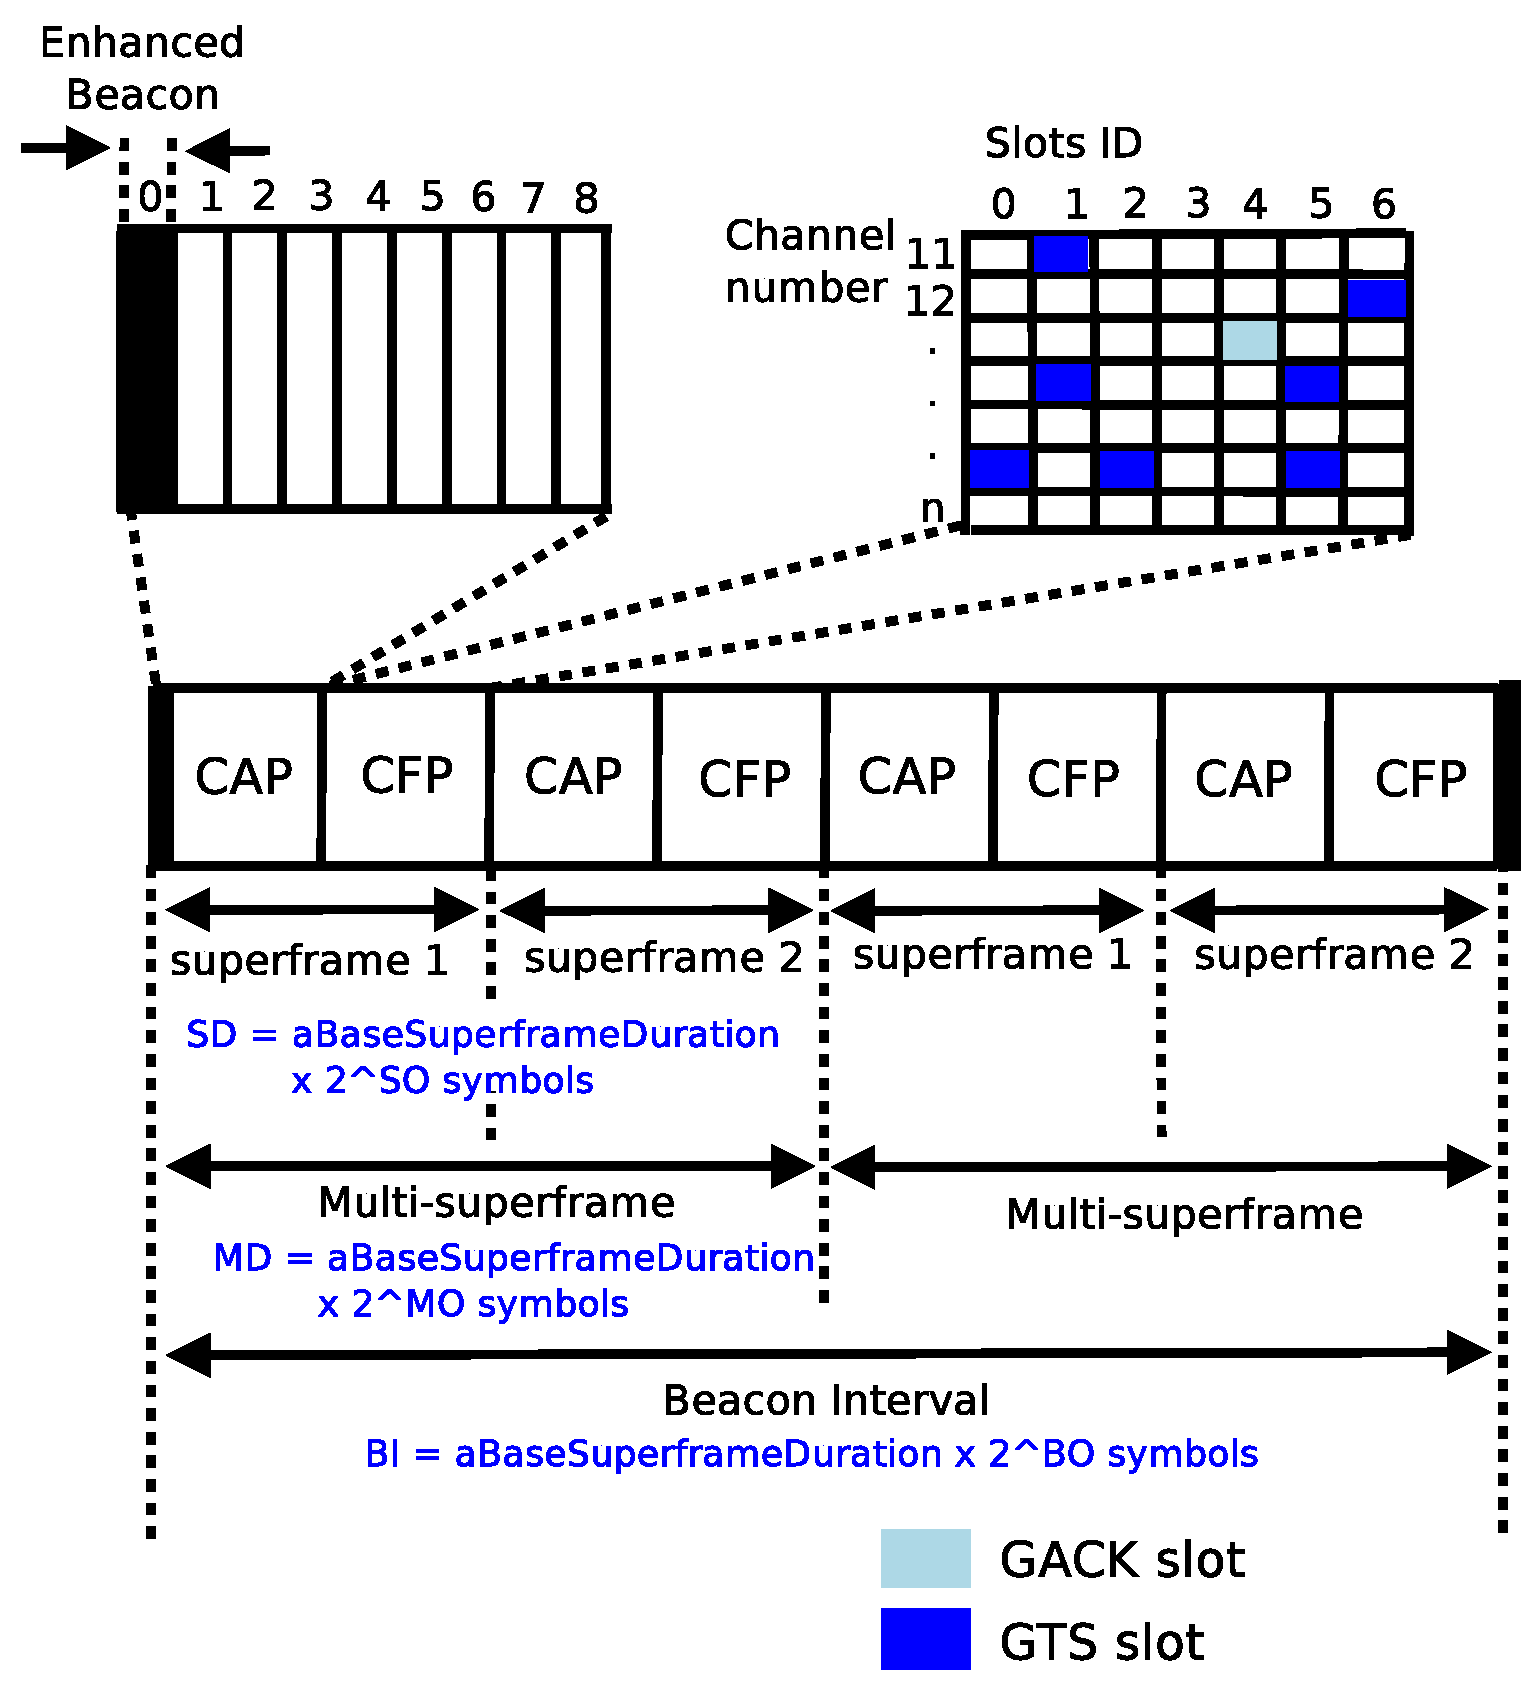
\includegraphics[scale=.28]{dsmeSuperframe}
\caption{DSME multi-superframe structure.}
\label{fig:dsmeSuperframe}
\end{figure}

 Another unique feature of DSME is CAP reduction. Except for the first superframe CAP in the multi-frame, DSME can completely eliminate subsequent CAPs in the multi-frame and use the gained time to effectively increased the time in exclusive transmissions in the CFPs operations. DSME Beacon Interval (BI) is equal to \mbox{$aBaseSuperframeDuration$ x $2^{BO}$} symbols where $aBaseSuperframeDuration$ is equal to 960 symbols and the Beacon Order (BO) is an integer between 0 and 14. The superframe duration (SD) is equivalent to \mbox{$aBaseSuperframeDuration$ x $2^{SO}$} symbols, where SO is the superframe order and is related to the BO in \mbox{0 $\leq$ $SO$ $\leq$ $BO$ $\leq$ 14}. Likewise, the Multi-superframe Duration (MD) is the result of \mbox{$aBaseSuperframeDuration$ x $2^{MO}$} symbols where MO is the Multi-superframe Order and relates to both SO and BO in \mbox{0 $\leq$ $SO$ $\leq$ $MO$ $\leq$ $BO$ $\leq$ 14}. To overcome interference as a result of noise present in a given channel, DSMA can check the link quality and use a \textit{channel adaptation} to switch a GTS (assigned to a specific device) to a different channel in a consecutive time slot. On the other hand, \textit{channel hopping}, a well known technique, can be used to set a predefined sequence to hop between channel during the whole frame transmission.

\textbf{LLDN}. The Low Latency Deterministic Networks MAC behavior was specifically designed for factory automation or implementations with similar requirements and limitations. LLDN is exclusive for centralized networks (star topology) that require latency as low as 10 ms for more than a 100 devices connected to a single coordinator. Examples of LLDN applications include but are not limited to robots, airport logistics, conveyors, automatic packing, cargo, etc. 
\begin{figure}[!htb]
\centering
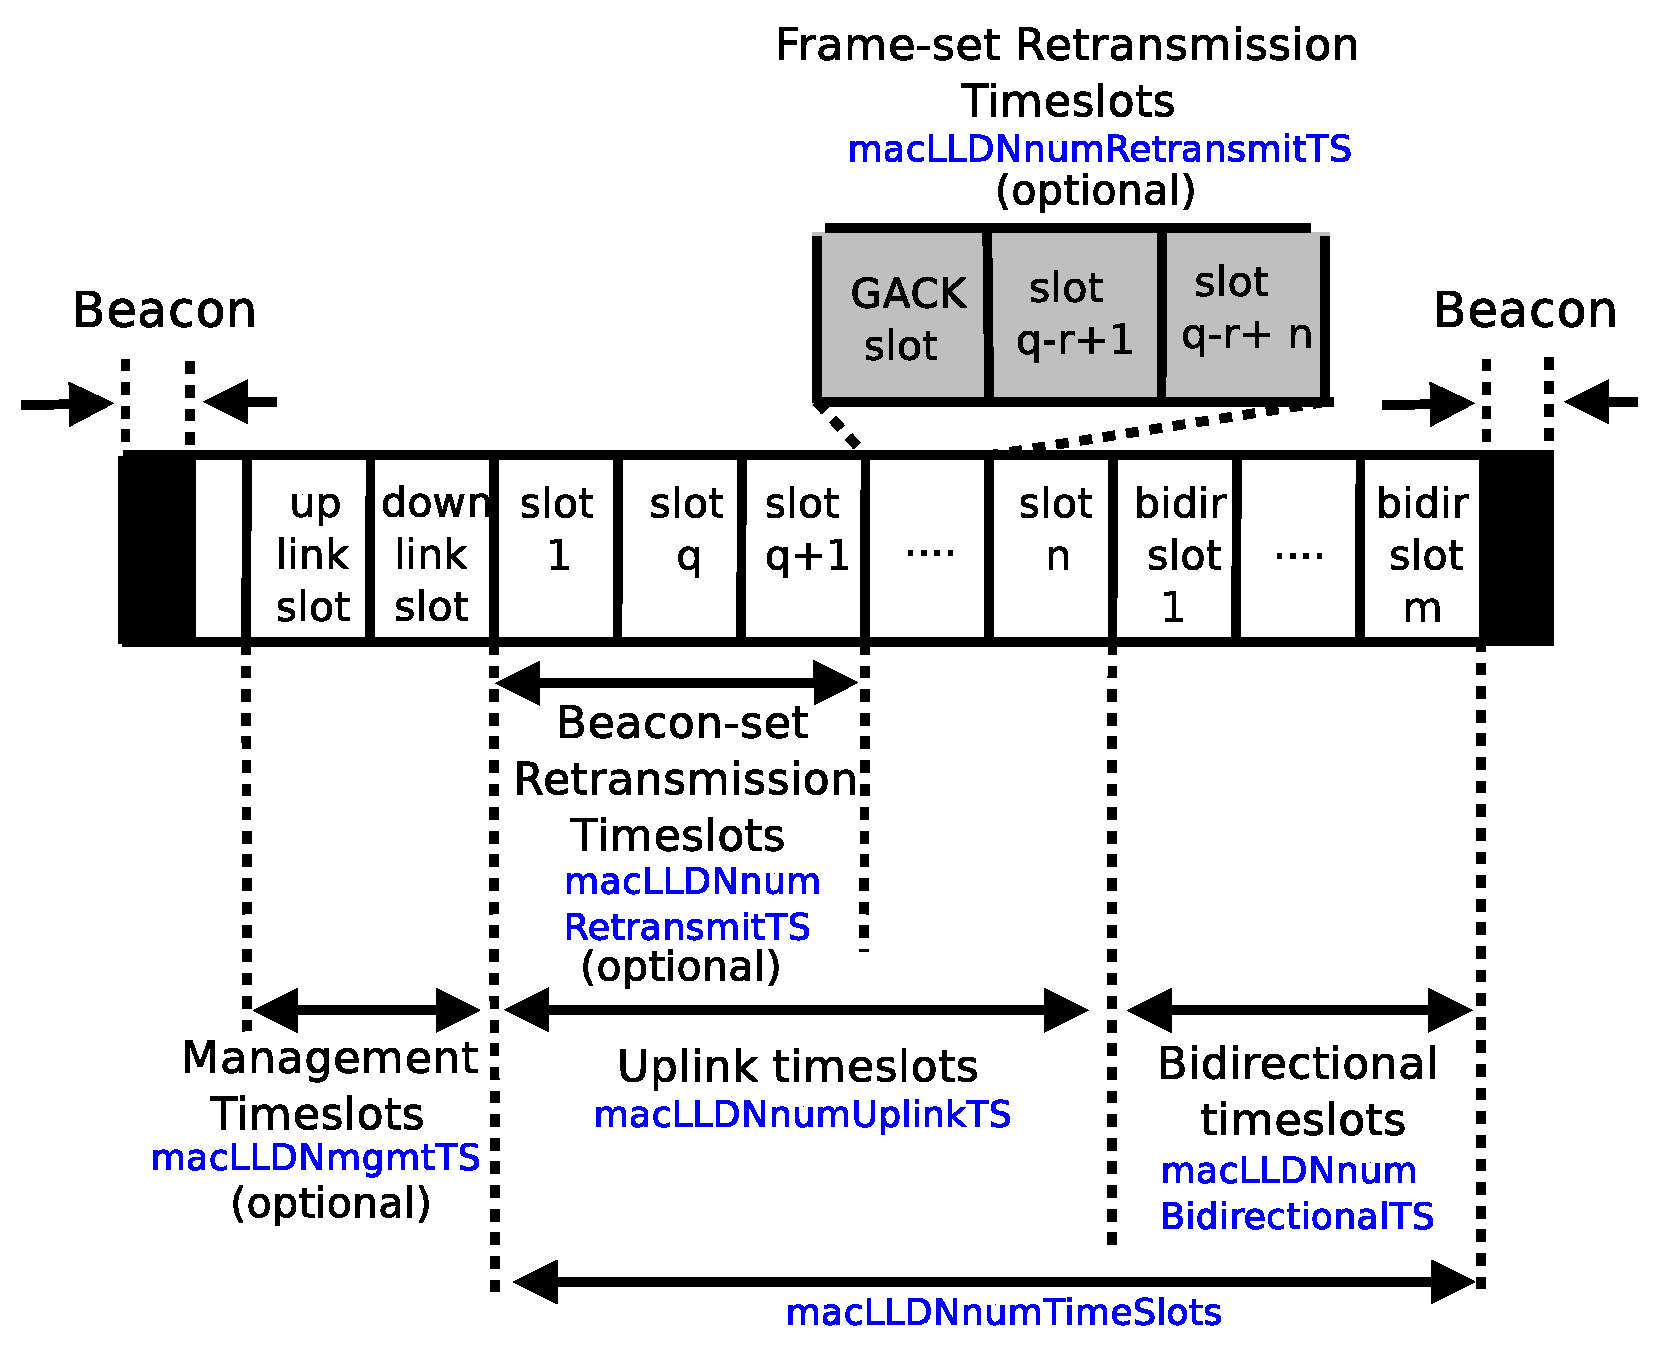
\includegraphics[scale=.28]{llframe}
\caption{LLDN superframe structure.}
\label{fig:llframe}
\end{figure}

In LLDN there can be two types of device; devices that can only send data to the coordinator (uplink capable) or devices that can do both, send and receive data from the coordinator (uplink and downlink capable). LLDN has a \textit{superframe} structure in which the first time slot is assigned to the beacon and the remaining slots of equal size are assigned to specific devices in the network. Multiple devices can be assigned to a single slot, in which case they contend for the medium using CSMA/CA. In LLDN, superframe time slots have a specific order and purpose: a) The \textit{beacon timeslot} which is always present. b) The \textit{management timeslots}: \textit{downlink} and \textit{uplink} timeslots. Management slots existence is optional and depends on whether or not the \textit{macLLDNmgmtTS} flag is set true. c) The \textit{uplink timeslots} are used for transmissions from the devices to the coordinator. Additionally, the first uplink slots can be used for re-transmissions if specified by the Group Acknowledgment (GACK) field contained in the beacon. Alternately, re-transmissions can also be set using a LL-Acknowledgment frame (command frame) sent in the \textit{bidirectional timeslots}.  d) \textit{Bidirectional timeslots} are used for multi-link communication between the coordinator and its devices. The slot size and number of slots for each usage are indicated by the \textit{macLLDN} attributes as shown in Figure \ref{fig:llframe}.

\textbf{TSCH}. The Time Slotted Channel Hopping MAC behavior was created with robustness in mind. TSCH applications include oil and gas industry, chemical and pharmaceutical production or applications prone to collisions caused by the saturation of the network. TSCH considers a deterministic response as the most important aspect of the communication. Different to DSME, TSCH support mesh as well as star topologies. In TSCH, \textit{superframes} are replaced with \textit{slotframes}. Slotframes repeat cyclically and are formed by a sequences of \textit{timeslots}. Each timeslot has an incremental Absolute Slot Number (ASN) that distinguishes it from one another. Transmissions inside these timeslots can take place with or without contention. Also, in TSCH, it is possible to use concurrent slotframes, each with independent timeslots configurations. However, all slotframes are aligned to the same timeslot boundaries.
Unlike the channel diversity used in DSME, TSCH relies on a channel hopping mechanism to achieve communication.
The frequency $f$ used in a transmission between two nodes is defined by \mbox{$f= F[(ASN+ channel Offset) \% NChannels]$} where \textit{channel Offset} is an integer between 0 and 15, \textit{NChannels} is the the number of channels in used for the current network (0-15) and $F$ represents a lookup table. In this way, a different frequency is obtained for the same link in different time slots.
\begin{figure}[!htb]
\centering
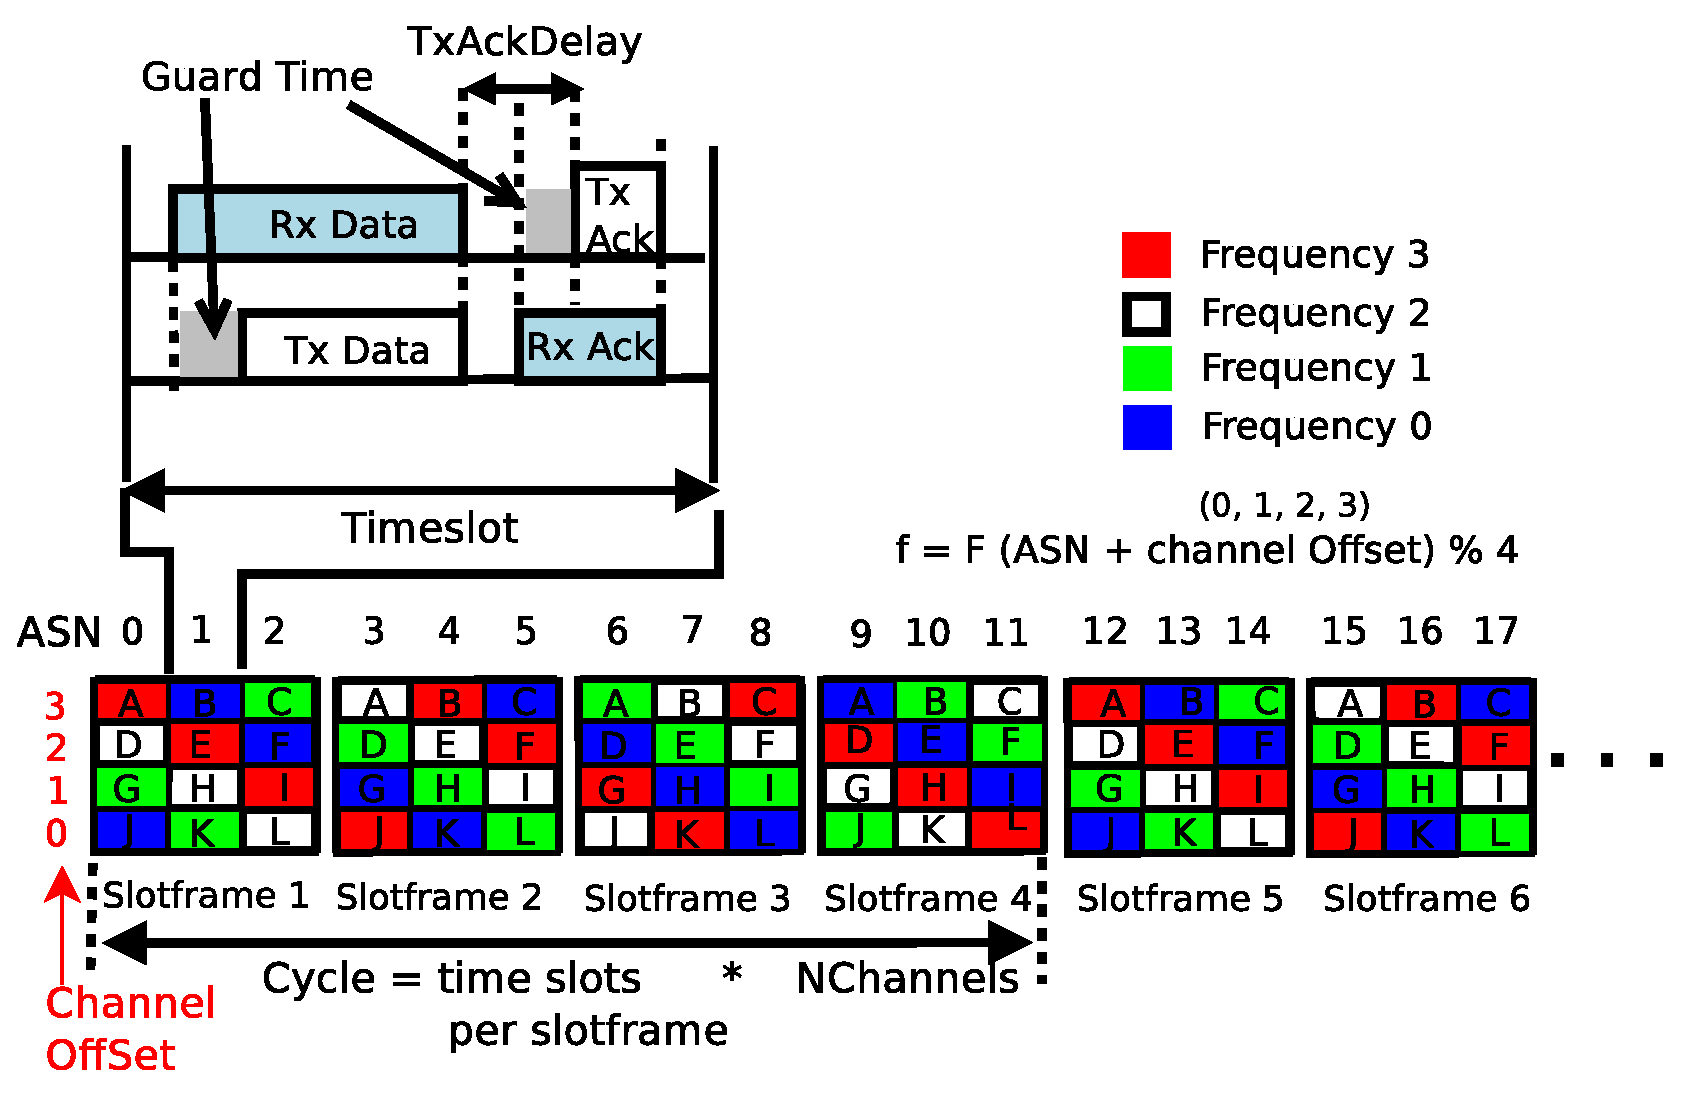
\includegraphics[scale=.28]{tschSlotframe}
\caption{TSCH concurret slotframe structure.}
\label{fig:tschSlotframe}
\end{figure}
\subsection{IEEE 802.15.4f (2012) - Amendment 2 }\label{wpan2012f}
 The 2nd amendment \cite{std2012f} to the 2011 revision has two new PHY. First, the Low rate PRF Ultra Wide Band (LRP UWB) optimized for low complexity RFID transmitters (tags) which has a level of interoperability  only present with the UWB PHY in previous revisions. LRP UWB offers 3 modes: a) \textit{Base mode} with an OOK modulation and a bit rate of 1000 kb/s. b) \textit{Extended mode}  with OOK modulation and a bit rate of 250 kb/s. c) \textit{Long-range mode} with a Manchester PPM modulation and a maximum bit rate of 31.25 kb/s. The second PHY is a 2450 MHz band PHY with a Minimum Shift Keying (MSK) modulation and a maximum bit rate of 250 kb/s targeted to RFID applications. The 2450 MHz band is the Industrial, Scientific and Medical (ISM) band and therefore, devices operate on it (e.g. Wi-fi, ZigBee). Despite this, there tend to be small unused gaps in the spectrum on the edges of these frequencies. MSK 2450MHz PHY take advantage of those spaces, and is capable of using up to 42 possible narrowband channels that fall on these unused gaps, gracefully coexisting with existing devices using the same band. Alternatively, MSK can operate on the much less saturated 433 MHz band with bit rates of 31.25, 100 or 250 kb/s.
\subsection{IEEE 802.15.4g (2012) - Amendment 3 }\label{wpan2012g}
IEEE 802.15.4g \cite{std2012g} know as the Smart Utility Networks (SUN) standard, was created to be used in the emerging Smart Grids (SG). SGs are electrical grids with the capacity of bidirectional energy flow and communication of signals\cite{smartGrid}. SUN PHYs are often used in smart metering applications with long-range, low-power requirements. This amendment introduces three PHY with multiple data rates to chose from. The PHY names are described by its modulations names: a) Multi-Rate and multi-regional Frequency Shift Keying (MR-FSK). b) Multi-Rate and multi-regional Offset Quadrature Phase-Shift Keying (MR-O-QPSK) that share characteristics with the 2011 modulation O-QPSK. c) The Multi-Rate and multi-regional Orthogonal Frequency Division Multiplexing (MR-OFDM) that use DSSS and MDSSS. Some of the SUN PHYs frequencies established in this amendment have been revised in later amendments.
\subsection{IEEE 802.15.4j (2013) - Amendment 4 }\label{wpan2014j}
This amendment \cite{std2013j} introduces a single PHY for the 2380 MHz band with a maximum bit-rate of 250 kb/s. Its use is restricted to the transmission data (no voice) in devices for monitoring, diagnosing and treating of patients. These devices must be compliant to the Federal Communications Commission (FCC) rules for Medical Body Area Networks (MBAN).
\subsection{IEEE 802.15.4k (2013) - Amendment 5 }\label{wpan2014k}
This amendment added 2 more PHYs: a) A DSSS PHY with either BPSK or O-QPSK modulation schemes. b) A FSK PHY with 3 possible modulations; a Gaussian FSK (GFSK), Position-based FSK (P-FSK) and Position-based Gaussian FSK (P-GFSK). These PHY are designed for Low Energy, Critical Infrastructure Monitoring (LECIM) applications. LECIM operates on a large number of frequencies \cite[pp. 58-61]{std2013k} with multiple data rate options for each one of these modulations. One of its main features is the possibility to use the priority channel access (PCA). PCA allows to allocate high priority messages in the CAP period of the superframe structure. Experiments conducted by Gebremedhin et al.\cite{experimentK} showed that under some conditions PCA messages can greatly improve the latency of emergency messages while just affecting slightly the performance of normal messages.
\subsection{IEEE 802.15.4m (2014) - Amendment 6 }\label{wpan2014m}
The amendment objective was to re-purpose the unused frequency space left between TV channels in UHF bands. Originally, this space was left unused to avoid TV channels interfering with one another. This space is known as TV White Space (TVWS) and its value lies in its potential for longer range communications. A 2.4 Ghz signal might travel several kilometers in the right conditions, however, UHF (470 - 698 MHz) can travel for many miles. However, it is worth noting that existent TVWS (i.e. 600 - 700 MHz) are increasingly becoming unavailable caused by the increasing demand of cellular frequencies. TVWS PHY support multiple data rates in bands ranging from 54 MHz to 862 MHz helped by 3 modulation schemes: TVWS-FSK, TVWS-OFDM, TVWS-NB-OFDM. IEEE 802.15.4m coexistence with other standards using TVWS have been explored in \cite{coexistance}.
\subsection{IEEE 802.15.4p (2014) - Amendment 7 }\label{wpan2014p}
This amendment \cite{std2014p} addressed the need for a communication standard in Rail Communications Control (RCC) systems. This standard enabled data rates of up to 1 Mbit/s over frequencies in the VHF, UHF, and SHF bands (161, 216, 217, 220, 450, 770, 896, 915, 928, 2450, 4965, 5800 MHz) operating in contiguous and non-contiguous channel bandwidths as narrow as 12.5 kHz and as wide as 2Mhz. The standard has multiple modulation technique options: GMSK, QPSK, DPSK among others. A full list of the frequencies and modulations introduced for this amendment can be found in \cite[pp. 386]{std2015}.
\subsection{IEEE 802.15.4 (2015) }\label{wpan2015}
IEEE 802.15.4-2015 \cite{std2015} is the third revision to the standard. As its predecessors, this collect all the PHYs additions and MAC enhancements since the 2011 revision in a single document. Additional corrections to the document are editorial in nature. 
\subsection{IEEE 802.15.4n (2016) - Amendment 1 }\label{wpan2016n}
The first amendment \cite{std2016n} to the 2016 revision present another PHY alternative for the transmission of medical information in China. The China Medical Band (CMB) defines the 174-216 MHz, 407-425 MHz and 608-630 MHz bands for this purpose and restricts its use for voice applications.
\subsection{IEEE 802.15.4q (2016) - Amendment 2 }\label{wpan2016q}
IEEE 802.15.4q \cite{std2016q} introduced two PHY for 2.4 GHz and multiple sub-gigahertz bands with data rates up to 1 Mb/s. These PHYs aimed to be ultra low-cost (low complexity) and ultra-low power. To achieve this, the standard used two new modulations: the Rate Switch Gaussian Frequency Shift Keying (RS-GFSK) and the Ternary Amplitude Shift Keying (TASK). RS-GFSK offered options to work along side existing SUN FSK PHYs. Consequently, smart metering, smart irrigation, home networks applications benefits from these PHYs.
\subsection{IEEE 802.15.4u (2016) - Amendment 3 }\label{wpan2016u}
This revision \cite{std2016u} takes many of the characteristics introduced in IEEE 802.15.4g and replicates them into the 866 band (865-867 MHz) to be used in creation of smart cities in India (smart grid, home control and security, etc). This standard defines 3 new PHYs corresponding to its modulations: MR-FSK (also called SUN-FSK), MR-OFDM, MR-O-QPSK.
\subsection{IEEE 802.15.4t (2017) - Amendment 4 }\label{wpan2017t}
A new PHY is introduced in this amendment \cite{std2017t} designed to operate on devices that require of short burst of information at high speeds (up to 2 Mb/s) followed by long sleep periods which results in a extended battery life. This amendment uses the the same 2400-483.5 MHz frequencies occupy by the O-QPSK PHY but it uses a MSK modulation instead.
\subsection{IEEE 802.15.4v (2017) - Amendment 5 }\label{wpan2017v}
This amendment \cite{std2017v} changed multiple SUN PHY frequency ranges as well as their channel rages. The changes conceded the use of the 870-876 MHz and the 915-921 Mhz in Europe, the 902-928 MHz in Mexico, the 902-907.5 in Brazil and the 915-928 MHz in Australia, Brazil and New Zealand. Additionally, frequency range changes are done to the LECIM and TVWS PHYs.
\subsection{IEEE 802.15.4s (2018) - Amendment 6 }\label{wpan2018s}
IEEE 802.15.4s \cite{std2018s} is the last amendment to the date. In this amendment, several MAC layer primitives and commands are added as part of the Spectrum Resource Measurements (SRM) toolkit. These changes are the most significant additions to the MAC layer since 802.15.4e-2012. SRM permits to measure, transmit or request information regarding the state of the channel. The MAC layer is able to report this information to higher layers for its usage. Some of the SRM introduced features are:





\begin{itemize}
  \setlength{\itemsep}{1pt}
  \setlength{\parskip}{0pt}
  \setlength{\parsep}{0pt}
  \item \textit{Failed Transmissions measurement.} It estimates the propagation quality of specific link as part of the channel selection algorithm.
  \item \textit{Deferred Transmissions measurement.} It helps to determinate the level of congestion in the channel caused by other coexisting networks.
  \item \textit{Retry Histogram.} It gives a histogram with the number of retries from a single transmission during a determinate space of time.
  \item \textit{Noise Histogram.} Reports the noise power of non-IEEE 802.15 devices in a specific channel during a specify period of time.  
  \item \textit{Channel Usage.} Show the total Channel time used during a sequence of Rx and Tx frames during a period of time.
  \item \textit{Received Signal Strength Indicator (RSSI)}
  \item \textit{Energy Detection (ED).}
\end{itemize}

Table \ref{tab:phyTable} summarize all the standard PHYs with its modulations, symbol rate and bit rate, except for the extensive LECIM, SUN and TVWS PHYs which are constantly changed.

 %[\begin{table}!htbp]
\begin{table}[!htbp]
%\begin{center}
\caption{IEEE 802.15.4 PHY evolution.}
\label{tab:phyTable}
{\renewcommand{\arraystretch}{1.2}
\begin{tabular}{|c|@{}c@{}|@{}c@{}|@{}c@{}|@{}c@{}|@{}c@{}|}
\hline
 \begin{tabular}{@{}c@{}}\textbf{PHY}\\ \textbf{(MHz)}\end{tabular} & 
 \begin{tabular}{@{}c@{}}\textbf{Band} \\ \textbf{(MHz)}\end{tabular} & 
 \begin{tabular}{@{}c@{}}\textbf{\scalebox{0.8}{Modulation -}} \\ \textbf{\scalebox{0.8}{Spread Spectrum}}\end{tabular} &  
 \begin{tabular}{@{}c@{}}\textbf{Bit-Rate}\\\textbf{(kb/s)}\end{tabular} & 
 
 \begin{tabular}{@{}c@{}}\textbf{Symbol}\\\textbf{Rate} \\ \textbf{(ksym/s)}\end{tabular} \\ \hline
 
 
 \begin{tabular}[c]{@{}c@{}}2450 \scalebox{0.8}{(World Wide)} \\ \scalebox{0.8}{IEEE 802.15.4-2003}\end{tabular} &  \begin{tabular}{@{}c@{}} 2400 - \\ 2483.5\end{tabular} & O-QPSK \scalebox{0.8}{*DSSS} & 250 & 62.5 \\ \hline





915 \scalebox{0.8}{(U.S.A)}  & 902 - & BPSK & 40 & 40 \\ \cline{3-5}
\scalebox{0.8}{IEEE 802.15.4-2003} & 928 & ASK \scalebox{0.8}{*PSS}& 250 & 50 \\ \cline{3-5}
     &   & O-QPSK & 250 & 62.5 \\ \hline





868 \scalebox{0.8}{(Europe)}  & 868 - & BPSK & 20 & 20 \\ \cline{3-5}
\scalebox{0.8}{IEEE 802.15.4-2003} & 868.6 & ASK \scalebox{0.8}{*PSS}& 250 & 12.5 \\ \cline{3-5}
     &   & O-QPSK & 100 & 25 \\ \hline

              
 
2450   & 2400-2483.5 & DQPSK$\,\to\,$  & 250 / &  166.667 / \\
\scalebox{0.8}{IEEE 802.15.4a-2007} &    & DQCSK \scalebox{0.8}{*CSS} & 1000         &                166.667 \\
\hline 

   
   
  
   
UWB sub-Ghz  & 250-750    &          & 110/850& \scalebox{0.8}{0.12/0.98(Mhz)}  \\
\cline{4-5}
sub-Ghz/low/high & 3244-4742  & BPM-BPSK & 6810 & 7.80(Mhz)  \\
\cline{4-5}
\scalebox{0.8}{IEEE 802.15.4a-2007} & 5944-10234 &          & 27240& 15.60(Mhz)  \\
\hline   
   
   
   
 780 \scalebox{0.8}{(China)}\    
 & 779 - & O-QPSK & 250 & 62.5 \\ \cline{3-5}
\scalebox{0.8}{IEEE 802.15.4c-2009} 
&787 & MPSK & 250 & 62.5 \\ \hline

    

 950 \scalebox{0.8}{(Japan)}\    
 & 950 -& GFSK & 100 & 100 \\ \cline{3-5}
\scalebox{0.8}{IEEE 802.15.4d-2009} 
&956  & BPSK \scalebox{0.8}{*DSSS}  & 20 & 20 \\ \hline



433 / 2450 & 433.05-434.79 & MSK & \scalebox{0.8}{31.25/100/250}& \scalebox{0.8}{31.25/100/250}  \\ 
\cline{2-2}\arrayrulecolor{white}\cline{3-3}\arrayrulecolor{black}\cline{4-5}
\scalebox{0.8}{IEEE 802.15.4f-2012} & 2400-2483    &     & 250 &250 \\
% \multicolumn{1}{r|}{250} & \multicolumn{1}{r|}{250}  \\
\hline   
   
   
   
  
 LRP UWB & 6289.6- & PPM & 31.25                         & 31.25            \\ 
\cline{3-5}
\scalebox{0.8}{IEEE 802.15.4f-2012} & 9185.6  & OOK & 250/1000 & 250/1000\\
\hline 
  
  
  
\begin{tabular}{@{}c@{}} 2380 \\ \scalebox{0.8}{IEEE 802.15.4j-2013}\end{tabular}   & 
\begin{tabular}{@{}c@{}} 2360 - \\ 2400\end{tabular}  
&O-QPSK \scalebox{0.8}{*DSSS}& 250 & 62.5 \\ \hline  
 

 



 195 / 416 / 619& 174-216 & \multirow{2}{*}{GFSK} & \multirow{2}{*}{50/100/200} & \multirow{2}{*}{50/100/200}  \\
\scalebox{0.8}{(China)} & 407-425 &   &   &      \\ 
\arrayrulecolor{white}\cline{2-2}\arrayrulecolor{black}\cline{3-5}
 \scalebox{0.8}{IEEE 802.15.4n-2016} & 608-630 & O-QPSK & 250/500    & 62.5/125 \\
\hline



   
   
   
                          &         & MR-FSK(2FSK)& 50/100/150              & 50/100/150  \\ 
\cline{3-5}
866 \scalebox{0.8}{(India)} &         & MR-OFDM   & 50/100/150              &             \\
\scalebox{0.8}{IEEE 802.15.4u-2016}& 865-867 &           & 200/300                 &             \\ 
\cline{3-5}
                          &         & MR-O-QPSK & 6.25/12.5/25            &   100/200          \\
                          &         & \scalebox{0.8}{*DSSS}          & 50 &             \\
\hline   
   
      
\begin{tabular}{@{}c@{}} 2450 \\ \scalebox{0.8}{IEEE 802.15.4t-2017}\end{tabular}   
& 
\begin{tabular}{@{}c@{}}2400-\\2483.5\end{tabular}   
  & MSK & 2000 & 250  \\ \hline 
    
    
       
\end{tabular}
}
%\end{center}
\end{table}



\section{IEEE 802.15.4 implementations} \label{implementationStd}
At times, simulations accuracy results can be questionable, however, without them large scale and costly experiments could not be conducted. The IEEE 802.15.4 is a popular protocol with multiple revisions. Despite this popularity, new revisions are slowly adopted. By far, the 2003 and 2006 revisions are the most implemented. 2012 revisions or later, brought highly specialized PHYs and MAC behaviors limited to specific industries and applications. Their implementation in simulations is somehow rare in comparison to the legacy standard. Examples of popular IEEE 802.15.4 implementations are as follows: 

The Ns-2 WPAN  module \cite{ns2implementation} is among the first simulations of the standard. Its latest version (2.35)  has a full support of the IEEE 802.15.4-2003, and is to the date, one of the most complete implementations of the standard with beacon and non-beacon support for mesh and star topologies (No support for inactive periods). Unfortunately, it suffers of some problems inherited from ns-2; lack of documentation and coding standards, unrealistic packet formats, unnecessary overhead and lack of maintenance. Its modules are coded using C++ while scenarios require OTcl scripting language.

 Castalia (v3.3) \cite{castalia} is an OMNET++ based simulator. Besides the basic 802.15.4-2006 MAC standard, Castalia support 3 more MAC layers: TunableMac, TMAC and IEEE 802.15.6. Castalia only has support for a beacon-enabled mode in a star topology with the optional GTS (No support for non-beacon, Indirect-transfers or mesh topology). Castalia has support for PHYs modulations QPSK, BPSK, PSK and FSK non present in the 2006 revision of the standard. C++ and NED languages are used in OMNET++ modules. 
 
  Ns-3 \cite{ns3} is a simulator with an active community developing new modules. Some of these modules even have emulation and hardware integration support. Ns-3 latest version (V3.29) LR-WPAN module supports a full PHY  IEEE 802-15.4-2006 set with non-beacon mode MAC for start topology PAN (No association or beacon-enabled mode MAC options). The module is promising, however, the module is still too limited in comparison to other simulators. Its code base is C++ with support for Python bindings.

The OPNET simulator provides an IEEE 802.15.4-2003 model \cite{opnet} with support for beacon-enabled mode in star topology (No support for association, Non beacon-enabled mode or mesh topology). Similar to OMNET++, it provides a robust GUI with the possibility to use Proto-C, C or C++ for its modules construction. OPNET major drawback is the requirement of a license.

OpenZB \cite{openzb} is an open source, real hardware implementation of the IEEE 802.15.4-2003 with beacon-enabled mode for star and mesh topologies on CrossBow MICAz and TelosB motes. OpenZB is completely programmed in nesC language (TinyOS).


\section{Conclusions} \label{conclusions}
In this paper we presented a historical compendium of the IEEE 802.15.4, a popular wireless standard. From it humble beginnings the standard have evolved and extended to better support monitoring, medical and train communications applications, and in recent times, PHYs for grid networks. Despite being yearly revised, our research shows that simulations and hardware implementations of the standard are rarely complete and even popular simulators do not include the most recent and specialized revisions of the standard. Future IoT networks performance will depend on network specialist choosing the right standard for the job and weather or not these standards support a smooth coexistence with other networks. With literally thousands of possible combinations to chose from, these specialist will have depend more on simulations and a careful selection of the network features.  
 

 

 

\bibliographystyle{IEEEtran}
\bibliography{evolution802_15}





























\end{document}
